% 简洁风格：浅色背景 + 细边框 + 行号 + 自动换行
\definecolor{codebg}{RGB}{248,249,250}
\definecolor{codeframe}{RGB}{220,223,228}
\definecolor{codekw}{RGB}{25,85,145}
\definecolor{codecm}{RGB}{90,125,90}
\definecolor{codestr}{RGB}{136,44,136}

\lstdefinestyle{cleancpp}{
	language=C++,
	basicstyle=\ttfamily\small,
	keywordstyle=\bfseries\color{codekw},
    commentstyle=\color{codecm},
	stringstyle=\color{codestr},
	backgroundcolor=\color{codebg},
	frame=single,
	rulecolor=\color{codeframe},
	framesep=6pt,
	numbers=left,
	numberstyle=\scriptsize\color{gray},
	numbersep=8pt,
	breaklines=true,
	breakatwhitespace=false,
	showstringspaces=false,
	keepspaces=true,
	tabsize=4,
	columns=fullflexible
}

\chapter{第一题}

\section{题目}

假设某科学计算程序在单核上的执行时间为 $T_{serial}=2000$ 秒。该程序中 90\% 的计算任务可以完全并行化。现将其部署在拥有 $p$ 个处理器的分布式集群上。经实测，该算法在并行化后会产生额外的通信延迟，延迟时间与处理器数量的关系公式为 $T_{comm}=0.05\times p^2$ 秒（此开销属于非并行部分）。

\begin{enumerate}
    \item 若不计通信延迟，根据阿姆达尔定律计算该程序在 $p=4,8,16$ 时的理论加速比。
    \item 计入通信延迟 $T_{comm}$ 后，写出并行运行时间 $T_{parallel}$ 随 $p$ 变化的数学表达式。
    \item 计算在计入通信延迟的情况下，处理器数量 $p$ 取何值时能获得最大加速比？此时的加速比是多少？
\end{enumerate}

\section{解答}

\subsection{第一问}
根据阿姆达尔定律，加速比的计算公式为：
$$ T_{parallel} = \frac{f \times T_{serial}}{p} + (1-f) \times T_{serial}  + T_{comm} $$

因为不考虑通信延迟，所以 $T_{comm}=0$，因此加速比 $S(p)$ 可以简化为：

$$ S(p) = \frac{T_{serial}}{T_{parallel}} =\frac{1} {\frac{f}{p} + (1-f)}$$
其中，$f$ 是程序中可以并行化的部分所占的比例，这里 $f=0.9$。

计算在 $p=4,8,16$ 时的加速比：
\begin{enumerate}
    \item 当 $p=4$ 时：
    $$ S(4) = \frac{1}{(1-0.9) + \frac{0.9}{4}} = \frac{1}{0.1 + 0.225} = \frac{1}{0.325} \approx 3.077 $$
    \item 当 $p=8$ 时：
    $$ S(8) = \frac{1}{(1-0.9) + \frac{0.9}{8}} = \frac{1}{0.1 + 0.1125} = \frac{1}{0.2125} \approx 4.706 $$
    \item 当 $p=16$ 时：
    $$ S(16) = \frac{1}{(1-0.9) + \frac{0.9}{16}} = \frac{1}{0.1 + 0.05625} = \frac{1}{0.15625} = 6.4 $$
\end{enumerate}

\subsection{第二问}
计入通信延迟后，总的并行运行时间 $T_{parallel}$ 由三部分组成：不可并行部分的运行时间、并行部分的运行时间以及通信开销。
\begin{itemize}
    \item 不可并行部分的运行时间：$T_{serial} \times (1-f) = 2000 \times (1-0.9) = 200$ 秒。
    \item 并行部分的运行时间：$\frac{T_{serial} \times f}{p} = \frac{2000 \times 0.9}{p} = \frac{1800}{p}$ 秒。
    \item 通信延迟：$T_{comm} = 0.05 \times p^2$ 秒。
\end{itemize}
因此，并行运行时间 $T_{parallel}$ 随处理器数量 $p$ 变化的数学表达式为：
$$ T_{parallel}(p) = 200 + \frac{1800}{p} + 0.05 p^2 $$

\subsection{第三问}
为了获得最大加速比，我们需要找到使并行运行时间 $T_{parallel}(p)$ 最小的处理器数量 $p$。为此，我们对 $T_{parallel}(p)$ 关于 $p$ 求导，并令导数为零：
$$ \frac{d T_{parallel}(p)}{dp} = -\frac{1800}{p^2} + 0.1 p $$
令 $\frac{d T_{parallel}(p)}{dp} = 0$，则有：
$$ 0.1 p = \frac{1800}{p^2} $$
$$ p^3 = \frac{1800}{0.1} = 18000 $$
$$ p = \sqrt[3]{18000} \approx 26.207 $$
由于处理器数量 $p$ 必须为整数，我们需要比较 $p=26$ 和 $p=27$ 时的并行运行时间：
\begin{itemize}
    \item 当 $p=26$ 时：
    $$ T_{parallel}(26) = 200 + \frac{1800}{26} + 0.05 \times 26^2 = 200 + 69.23 + 33.8 = 303.03 \text{ 秒} $$
    \item 当 $p=27$ 时：
    $$ T_{parallel}(27) = 200 + \frac{1800}{27} + 0.05 \times 27^2 = 200 + 66.67 + 36.45 = 303.12 \text{ 秒} $$
\end{itemize}
比较可知，$T_{parallel}(26) < T_{parallel}(27)$，因此当 $p=26$ 时能获得最小的并行运行时间，从而得到最大加速比。
此时的最大加速比为：
$$ S_{max} = \frac{T_{serial}}{T_{parallel}(26)} = \frac{2000}{303.03} \approx 6.600 $$
所以，当处理器数量为 26 时，能获得最大加速比，约为 6.600。

\chapter{第二题}

\section{题目}

下面是一段简单的代码，试分析在单核模式下和多核模式下的性能对比：假设核心数为 8，并行计算时负载均衡，采用树形规约，每次计算耗时和规约耗时均相同，时间均为 $t$，分析完成整个计算时，单核与多核情况下主核分别进行了多少次运算，两者完成整个计算耗时对比，并简单画出多核计算时的树形图或者示意图。

\begin{lstlisting}[style=cleancpp]
int total_sum=0;
    for(int i=1;i<=32;i++){
        total_sum+=i*2;
}
\end{lstlisting}

\section{解答}

\subsection{基本概念}
\begin{itemize}
    \item 树形规约(Tree Reduction)：这是一种将数据集逐步合并的方法，常用于并行计算中。比如求和操作，可以将数据分成几部分并行计算各自的和，然后将这些中间结果再次两两合并，直到得到最终的结果。
    \item 负载均衡(Load Balancing)：确保所有核心的工作量尽可能相等，避免某些核心过度工作而其他核心闲置的情况。
\end{itemize}

\subsection{单核情况}
在单核模式下，循环体需要执行 32 次。每次循环包含一次乘法和一次加法。我们视作一次“计算”。
\begin{itemize}
    \item \textbf{主核运算次数}：主核（即唯一的计算核心）需要独立完成所有 32 次计算。
    \item \textbf{总耗时}：由于每次计算耗时为 $t$，总耗时为 $32t$。
\end{itemize}

\subsection{多核情况}
在多核模式下，我们有 8 个核心可以并行处理。
\begin{itemize}
    \item \textbf{并行计算阶段}：32 次计算被平均分配给 8 个核心，每个核心负责 $32 / 8 = 4$ 次计算。由于是并行执行，这个阶段的耗时为 $4t$。
    \item \textbf{树形规约阶段}：8 个核心计算出的局部和需要通过树形规约（Tree-based Reduction）合并。
    \begin{itemize}
        \item \textbf{第一轮规约}：8 个局部和两两相加，需要 $8/2=4$ 次规约操作。这 4 次操作可以并行进行，耗时为 $t$。此时剩下 4 个中间结果。
        \item \textbf{第二轮规约}：4 个中间结果两两相加，需要 $4/2=2$ 次规约操作，耗时为 $t$。此时剩下 2 个中间结果。
        \item \textbf{第三轮规约}：最后 2 个结果相加，需要 1 次规约操作，耗时为 $t$。得到最终总和。
    \end{itemize}
    整个规约过程共需要 $\log_2(8) = 3$ 轮，总耗时为 $3t$。
    \item \textbf{主核运算次数}：在并行计算阶段共执行了 4 次计算。在树形规约阶段，主核需要参与每一轮的规约操作，共 3 次。因此，总共进行了 $4 + 3 = 7$ 次运算。
    \item \textbf{总耗时}：总耗时为并行计算时间加上规约时间，即 $4t + 3t = 7t$。
\end{itemize}

\subsection{性能对比}
\begin{itemize}
    \item \textbf{主核运算次数对比}：单核情况下为 32 次，多核情况下为 7 次。
    \item \textbf{总耗时对比}：单核情况下为 $32t$，多核情况下为 $7t$。加速比为 $32t / 7t \approx 4.57$。
\end{itemize}

\subsection{树形规约示意图}
下图展示了 8 个核心进行树形规约的过程。S0 到 S7 代表 8 个处理器核心，它们各自计算出局部和（$S_i$-$S_j$），然后分三轮进行合并。

\begin{figure}[h]
    \centering
    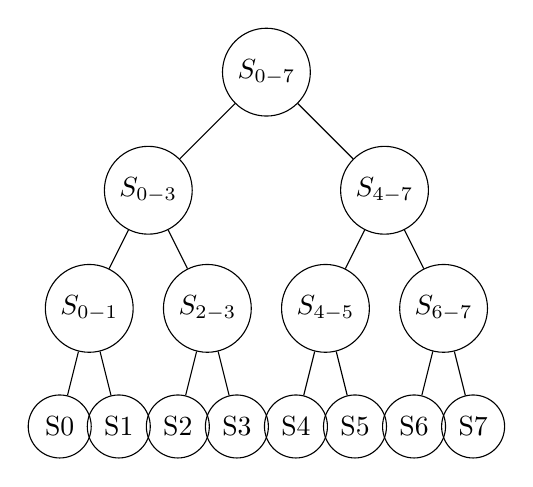
\begin{tikzpicture}[
        level 1/.style={sibling distance=3cm, level distance=1.5cm},
        level 2/.style={sibling distance=1.5cm, level distance=1.5cm},
        level 3/.style={sibling distance=0.75cm, level distance=1.5cm},
        every node/.style={draw, circle, minimum size=0.8cm}
    ]
    \node (sum) {$S_{0-7}$}
        child { node (s03) {$S_{0-3}$}
            child { node (s01) {$S_{0-1}$}
                child { node (s0) {S0} }
                child { node (s1) {S1} }
            }
            child { node (s23) {$S_{2-3}$}
                child { node (s2) {S2} }
                child { node (s3) {S3} }
            }
        }
        child { node (s47) {$S_{4-7}$}
            child { node (s45) {$S_{4-5}$}
                child { node (s4) {S4} }
                child { node (s5) {S5} }
            }
            child { node (s67) {$S_{6-7}$}
                child { node (s6) {S6} }
                child { node (s7) {S7} }
            }
        };
    
    % \node[below=0.2cm of s0] {P0};
    % \node[below=0.2cm of s1] {P1};
    % \node[below=0.2cm of s2] {P2};
    % \node[below=0.2cm of s3] {P3};
    % \node[below=0.2cm of s4] {P4};
    % \node[below=0.2cm of s5] {P5};
    % \node[below=0.2cm of s6] {P6};
    % \node[below=0.2cm of s7] {P7};

    \end{tikzpicture}
    \caption{8核树形规约示意图}
\end{figure}

\chapter{第三题}

\section{题目}

考虑一个现代化的大规模异构超级计算机节点，其硬件配置如下：

主机端：包含 2 颗多核 CPU（每颗 64 核），支持 AVX-512 向量指令集。

加速端：挂载 4 张高性能 GPU 卡。

互联：CPU 与 GPU 之间通过 PCIe 5.0 连接，GPU 与 GPU 之间通过 NVLink 互联。

该节点正在运行一个大规模流体动力学模拟程序，请回答以下问题：

\begin{enumerate}
    \item 请分别指出以下三个层级在 Flynn 分类法中所属的类别：
    \begin{enumerate}
        \item 单个 CPU 核心执行 AVX-512 向量指令时。
        \item 单张 GPU 内部的数千个 CUDA 核心协同工作时。
        \item 整个节点（2 颗 CPU + 4 张 GPU）协同处理不同任务模块时。
    \end{enumerate}
    \item 在该流体模拟中，为了提高容错性，工程师提议让 3 个不同的 CPU 核心同时读取相同的输入数据流，分别运行三种不同的误差校正算法，最后通过投票机制输出结果，这一特定子任务属于 Flynn 分类法中的哪一类？学术界常争论 MISD 在现实中几乎不存在，请结合此案例反驳或支持该观点，并说明 MISD 架构在现代计算中的主要应用场景是什么？
    \item 传统的 Flynn 分类法将系统严格划分为四类，然而，现代超算节点通常被称为 MIMD-SIMD 混合架构，为什么不能简单地将整个节点归类为单纯的 MIMD 或 SIMD？
\end{enumerate}

\section{解答}

\subsection{第一问：Flynn 分类}
\begin{enumerate}
    \item \textbf{单个 CPU 核心执行 AVX-512 向量指令时}：属于 \textbf{SIMD (Single Instruction, Multiple Data)}。AVX-512 是一套向量指令集，允许单条指令同时对多个数据元素（例如一个 512 位的向量）执行相同的操作。
    \item \textbf{单张 GPU 内部的数千个 CUDA 核心协同工作时}：属于 \textbf{SIMD} 的一种变体，为 \textbf{SIMT (Single Instruction, Multiple Threads)}。在 CUDA 架构中，一组线程（一个 Warp）中的所有线程执行相同的指令，但作用于不同的数据。这本质上是 SIMD 的思想在多线程环境下的实现。
    \item \textbf{整个节点（2 颗 CPU + 4 张 GPU）协同处理不同任务模块时}：属于 \textbf{MIMD (Multiple Instruction, Multiple Data)}。该节点的不同处理单元（CPU 核心、GPU 卡）可以独立地执行不同的指令流，处理各自不同的数据。例如，CPU 可能负责数据预处理和任务调度，而不同的 GPU 可能同时运行不同的计算密集型内核。
\end{enumerate}

\subsection{第二问：MISD 架构分析}
\begin{enumerate}
    \item \textbf{子任务分类}：这个特定的子任务——让 3 个不同的 CPU 核心同时读取相同的输入数据流，并运行三种不同的误差校正算法——是 \textbf{MISD (Multiple Instruction, Single Data)} 的一个典型例子。这里有多个指令流（三种不同的算法），但它们都作用于同一个数据流（输入数据）。
    \item \textbf{关于 MISD 现实性的讨论}：
    \begin{itemize}
        \item \textbf{反驳“MISD 不存在”的观点}：这个案例本身就是对“MISD 在现实中几乎不存在”这一观点的有力反驳。它展示了一个非常实用的场景：通过执行多个不同的处理流程来处理同一份数据，以实现容错和结果验证。这种设计在航空航天、金融交易、关键安全系统等对可靠性要求极高的领域至关重要。
        \item \textbf{正面观点的依据}：纯粹的、通用的 MISD 计算机非常罕见。它不像 SIMD 和 MIMD 那样被广泛用于通用计算性能的提升。其应用领域相对狭窄和特定。
    \end{itemize}
    \item \textbf{MISD 架构的主要应用场景}：
    \begin{itemize}
        \item \textbf{容错计算}：如题目中的例子，通过 N模冗余（N-version programming）来提高系统的可靠性。
        \item \textbf{信号处理}：例如，多个不同的滤波器并行处理同一个输入信号流。
        \item \textbf{密码学}：尝试用多种不同的算法或密钥并行破解同一段密文。
    \end{itemize}
\end{enumerate}

\subsection{第三问：混合架构}
现代超算节点不能简单归类为单纯的 MIMD 或 SIMD，因为它们在不同层次上体现了不同的并行模式，是一种层次化的混合架构。
\begin{itemize}
    \item \textbf{MIMD}：在最高层级，整个节点是 MIMD 的。多颗 CPU 和多张 GPU 可以独立运行不同的程序或任务，它们之间是异步和独立的。这是典型的多指令、多数据流模式。
    \item \textbf{SIMD}：在每个处理单元内部，又存在 SIMD 模式。每个 CPU 核心可以通过其向量处理单元（如 AVX-512）执行 SIMD 操作。每张 GPU 内部的数千个核心以 SIMT (SIMD 的变体) 模式工作。
\end{itemize}
因此，将整个节点称为 \textbf{MIMD-SIMD 混合架构} 是最准确的描述。它反映了现代高性能计算系统通过在不同粒度上组合多种并行策略来最大化计算能力的复杂现实。单纯归类为 MIMD 会忽略其核心计算单元（CPU向量单元和GPU）的 SIMD 特性；单纯归类为 SIMD 则完全错误，因为它忽略了多个处理单元可以独立执行不同任务的宏观并行性。


\chapter{第四题}

\section{题目}

考虑下图所示的搜索树，其中深色的节点表示问题的解

\begin{enumerate}
    \item 对树的串行搜索采用深度优先（DFS）算法，如果树的每个边耗费一个单位时间，那么需要多长时间才能找到解？
    \item 将树在两个处理器间进行分布，如图所示，共同完成搜索任务。如果两个处理器都在它们各自的树上进行 DFS 搜索（均从根节点开始），且两个处理器速度相当、均为每个边耗费一个单位时间，那么要找到解需要多长时间，加速比是多少？
\end{enumerate}

\begin{figure}
    \centering
    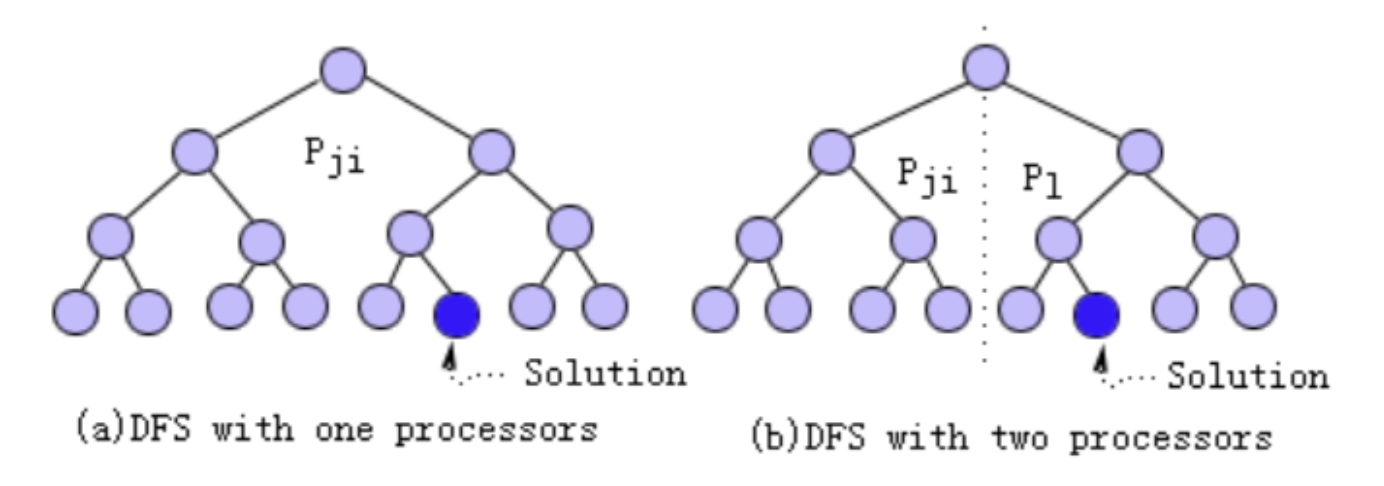
\includegraphics[width=\textwidth]{image/4-1.png}
    \caption{搜索树示例}
\end{figure}

\section{解答}

\subsection{第一问：串行搜索}
深度优先搜索（DFS）会沿着一条路径尽可能深地探索，直到到达叶子节点，然后回溯。假设搜索顺序为从左到右。
\begin{itemize}
    \item 搜索从根节点开始，首先进入左子树。
    \item 处理器会遍历完整个左子树。左子树包含 7 个节点，除了根节点外有 6 个节点，意味着需要向下遍历 7 条边（包含从根节点进入左子树），然后回溯 7 条边。总共是 $ 7 \times 2 = 14 $ 条边的 traversal。
    \item 从根节点向下进入右子树，耗时 1 个单位时间。
    \item 进入右子树后，首先访问其左侧分支。从 L1 节点到 L2 节点，耗时 1。
    \item 从 L2 节点继续向左探索，到达叶子节点，耗时 1。然后回溯，耗时 1。
    \item 从 L2 节点向右探索，到达深色的解节点，耗时 1。
\end{itemize}
所以，找到解所经过的总边数为：
$$ \text{总时间} = \underbrace{7}_{\text{L1左子树向下}} + \underbrace{7}_{\text{L1左子树回溯}} + \underbrace{1}_{\text{根到L1右}} + \underbrace{1}_{\text{L1右到L2左}} + \underbrace{1}_{\text{L2左到叶}} + \underbrace{1}_{\text{回溯到L2左}} + \underbrace{1}_{\text{L2左到解}} = 19 $$
因此，串行搜索需要 \textbf{19 个单位时间}才能找到解。

\subsection{第二问：并行搜索}
两个处理器 P0 和 P1 并行工作。
\begin{itemize}
    \item 处理器 P0 负责搜索左子树。
    \item 处理器 P1 负责搜索右子树。
\end{itemize}
两个处理器同时从根节点开始向下搜索，但分别进入不同的子树。
\begin{itemize}
    \item P0 进入左子树，开始它的 DFS 过程。
    \item P1 进入右子树，开始它的 DFS 过程。
    \item P1 的搜索路径为：根 -> L1右 -> L2左 -> L2左的左叶 -> 回溯 -> L2左的右叶（解）。
\end{itemize}
由于两个处理器是同时开始的，整个搜索的完成时间取决于最先找到解的那个处理器所花费的时间。
P1 找到解需要的时间为：
$$ \text{时间} = \underbrace{1}_{\text{根到L1右}} + \underbrace{1}_{\text{L1右到L2左}} + \underbrace{1}_{\text{L2左到叶}} + \underbrace{1}_{\text{回溯到L2左}} + \underbrace{1}_{\text{L2左到解}} = 5 $$
因此，并行搜索需要 \textbf{5 个单位时间}就能找到解。

\textbf{加速比} 的计算公式为：
$$ S = \frac{T_{serial}}{T_{parallel}} = \frac{19}{5} = 3.8 $$
加速比为 \textbf{3.8}。

\chapter{第五题}

\section{题目}

设有二维数组 $A[8][8]$，按行优先方式存放在内存中。假设 cache 一次可存放一整行数据。比较下面两段程序的访存行为。

程序一：
\begin{lstlisting}[style=cleancpp]
for (int i = 0; i < 8; i++) {
    for (int j = 0; j < 8; j++) {
        sum += A[i][j];
    }
}
\end{lstlisting}

程序二：
\begin{lstlisting}[style=cleancpp]
for (int j = 0; j < 8; j++) {
    for (int i = 0; i < 8; i++) {
        sum += A[i][j];
    }
}

\end{lstlisting}

请回答下列问题：
\begin{enumerate}
    \item 哪一段程序的缓存访问效率更高？为什么？
    \item 两段程序分别体现了怎样的空间局部性特征？
    \item 若数组规模进一步增大，而 cache 大小不变，两段程序的性能差异会如何变化？请简要说明理由。
\end{enumerate}

\section{解答}

\subsection{第一问：缓存效率}
\textbf{程序一}的缓存访问效率更高。

\textbf{原因}：
\begin{itemize}
    \item 数组 $A$ 是按\textbf{行优先}方式存放在内存中的，这意味着同一行中的元素（如 $A[i][j]$ 与$A[i][j+1]$）在内存地址上是连续的。
    \item \textbf{程序一}的访问顺序是 $A[i][j]$，其中内层循环遍历 $j$。这使得程序按顺序访问内存中连续的数据。当访问第一个元素 $A[i][0]$ 时，由于题目假设“cache 一次可存放一整行数据”，整个第 $i$ 行的数据都被加载到缓存中。接下来的 7 次访问（$A[i][1]$ 到 $A[i][7]$）将直接在缓存中命中（Cache Hit），无需再从主内存读取，速度非常快。对于 8x8 的数组，总共只需要 8 次主内存访问（每次加载一行），和 $8 \times 7 = 56$ 次缓存命中。
    \item \textbf{程序二}的访问顺序是 $A[i][j]$，但内层循环遍历 $i$。它访问的顺序是 $A[0][j]$ 到 $A[7][j]$。这些元素在内存中是不连续的，它们分别位于不同行的相同列上。每次访问 $A[i][j]$ 都会导致一次缓存未命中（Cache Miss），因为需要从主内存加载新的一行。例如，访问 $A[0][0]$ 加载第 0 行，紧接着访问 $A[1][0]$ 又需要加载第 1 行，导致刚刚加载的第 0 行数据可能被换出。因此，每次访问都可能是一次缓存未命中，总共可能导致 $8 \times 8 = 64$ 次缓存未命中。
\end{itemize}

\subsection{第二问：空间局部性}
\begin{itemize}
    \item \textbf{程序一}体现了\textbf{良好的空间局部性}。空间局部性原理指出，如果一个内存位置被访问，那么它附近的位置也很有可能在近期被访问。程序一按行遍历，其访存模式与数据在内存中的物理布局完全一致，完美地利用了空间局部性。
    \item \textbf{程序二}体现了\textbf{不好的空间局部性}。它按列遍历，每次访问都会跳过一大段内存（通常是一整行的长度）去访问下一行的同一个列元素。这种跳跃式的访问模式破坏了空间局部性。
\end{itemize}

\subsection{第三问：性能差异变化}
若数组规模进一步增大（例如变成 $A[N][N]$，其中 $N$ 远大于 8），而 cache 大小不变（例如 cache 仍然只能存放远小于 $N$ 个元素的一行或几行），两段程序的\textbf{性能差异会急剧扩大}。

\textbf{理由}：
\begin{itemize}
    \item 对于\textbf{程序一}（行主序遍历），其访存模式依然保持良好的空间局部性。只要 cache 能存下一部分行数据，它总能从每次内存加载中获得多次缓存命中。
    \item 对于\textbf{程序二}（列主序遍历），问题会变得极其严重。当外层循环遍历到下一列（$j+1$）时，内层循环需要重新从第一行（$i=0$）开始访问。由于数组规模很大，当程序访问到 $A[0][j+1]$ 时，之前为访问 $A[N-1][j]$ 而加载到 cache 的数据行很可能已经被换出。更糟糕的是，如果 cache 的大小连数组的一列都无法容纳，那么在内层循环中，每次访问 $A[i][j]$ 都可能会把 $A[i-1][j]$ 所在的数据块从 cache 中替换出去，导致几乎每次访问都是 Cache Miss。这种现象被称为\textbf{缓存抖动（Cache Thrashing）}，会造成性能的灾难性下降。
\end{itemize}
总结来说，随着数组规模增大，程序二的缓存未命中率会趋近于 100\%，而程序一则能继续保持较高的缓存命中率，因此二者的性能差距会变得越来越悬殊。

\chapter{第六题}

\section{题目}

某同学想测试程序 \texttt{test\_prog} 的运行时间，分别使用了两组输入数据 \texttt{input1} 和 \texttt{input2}，并使用 Unix shell 命令 \texttt{time} 得到如下结果：

对于 input1：
\begin{lstlisting}[style=cleancpp]
time ./test_prog < input1
real 0m0.002s
user 0m0.001s
sys 0m0.000s
\end{lstlisting}

对于 input2：
\begin{lstlisting}[style=cleancpp]
$ time ./test_prog < input2
real 0m1.532s
user 0m1.210s
sys 0m0.120s
\end{lstlisting}
其中，\texttt{real} 为程序从开始到结束的总耗时；\texttt{user} 为程序在用户态执行所消耗的 CPU 时间；\texttt{sys} 为程序在内核态执行所消耗的 CPU 时间，例如 I/O、系统调用等带来的时间。

请回答下列问题：
\begin{enumerate}
    \item 对于哪一组输入数据，更适合直接使用这种方式测量程序运行时间？为什么？
    \item 如果程序运行时间非常短，计时可能会遇到什么问题？应如何改进测量方法？
\end{enumerate}

\section{解答}

\subsection{第一问：选择合适的输入数据}
对于\textbf{input2}，更适合直接使用 \texttt{time} 命令测量程序运行时间。

\textbf{原因}：
\begin{itemize}
    \item \textbf{input1} 的运行时间太短了。\texttt{real} 时间只有 0.002 秒，\texttt{user} 时间只有 0.001 秒。如此短的时间间隔非常接近操作系统计时器的精度极限。这会导致测量结果有很大的\textbf{相对误差}，甚至可能是随机的。例如，单次运行的结果可能受到系统后台进程、中断等微小扰动的影响，使得结果非常不稳定。
    \item \textbf{input2} 的运行时间较长（\texttt{real} 1.532 秒），远大于计时器的精度。在这个时间尺度上，单次测量的结果相对稳定，能够更准确地反映程序的真实性能。系统噪声等瞬时因素对总时间的影响占比较小，因此测量结果更具\textbf{可信度}和\textbf{可复现性}。
    \item 此外，\texttt{user} 和 \texttt{sys} 时间之和（1.210s + 0.120s = 1.330s）与 \texttt{real} 时间（1.532s）有一定差距，这可能表明程序在等待 I/O 或在多核环境下存在并行，但总的来说，其 CPU 时间足够长，适合测量。
\end{itemize}

\subsection{第二问：短时间计时的改进方法}
如果程序运行时间非常短，直接计时会遇到以下问题：
\begin{itemize}
    \item \textbf{计时精度不足}：系统时钟的解析度有限（例如毫秒级），无法精确捕捉到微秒或纳秒级的事件。
    \item \textbf{测量开销占比过大}：启动进程、执行 \texttt{time} 命令本身也有开销，当被测程序运行时间极短时，这些测量开销可能会占总时间的很大一部分，从而扭曲结果。
    \item \textbf{结果不稳定}：容易受到操作系统调度、缓存状态、后台任务等随机因素的干扰，导致每次测量的结果波动很大。
\end{itemize}

\textbf{改进方法}：
\begin{enumerate}
    \item \textbf{重复执行多次}：最常用和最简单的方法是将需要测试的代码段放在一个\textbf{循环}中，执行成千上万次，然后测量整个循环的总时间。最后将总时间除以循环次数，得到单次执行的平均时间。这样可以有效地“放大”运行时间，使其远超计时器的精度，并平滑掉单次运行的随机波动。
    \item \textbf{使用高精度计时器}：使用操作系统或语言库提供的更高精度的计时函数，例如 C++ 和 POSIX 的一些库提供了工具能提供纳秒级别的计时精度。
    \item \textbf{预热（Warm-up）}：在正式计时前，先运行几次被测代码。这有助于确保指令和数据已经被加载到 CPU 缓存中，避免首次运行时的“冷启动”效应（如 JIT 编译、动态链接等）对测量结果造成影响。
\end{enumerate}
综合来看，对于 input1 这种情况，最佳实践是\textbf{在程序内部实现一个循环来重复执行核心逻辑，并使用高精度计时器来测量总耗时}，从而计算出可靠的平均单次运行时间。
